\chapter{Testing and CI}

Software development is not just about writing code that works; it is about writing code that \textit{continues} to work as the system evolves. When building non-trivial systems, the confidence a developer has in their codebase stems directly from the safety nets they have put in place. Testing is the primary safety net.

In this chapter, we will explore the philosophy behind automated testing, the mechanisms Rust provides to test your code natively, and how writing tests can fundamentally improve the design of your software.

\section{The Philosophy of Testing}

Imagine a manufacturing plant that produces plastic water bottles. The plant does not wait until a million bottles are shipped to customers to check if they hold water. Instead, there are quality control gates at every step of the production cycle. For instance, the water source is continuously analyzed to ensure no epidemics are spread. The raw plastic pellets are sampled for their chemical and physical characteristics before entering the machine---otherwise, the plant might produce 18,000 defective bottles. During the blow-molding phase, where recycled trimmings are sometimes used, a lack of material might cause a bottle to form incompletely (becoming just a deformed piece of plastic). Camera systems immediately discard these errors.

In software engineering, testing serves the exact same purpose. Many developers fall into the trap of writing a piece of code, running it once with a temporary \texttt{main} function to see if it prints the right output, and then moving on. However, this manual verification is lost to time. When the codebase grows, or when another developer modifies that code six months later, there is no automatic way to verify that the original behavior remains intact.

Writing tests is an investment in the future. It helps prevent \textbf{regressions}---bugs that occur when new additions unintentionally break existing functionality. They are also essential during \textbf{refactoring}: you must have a solid suite of tests for version 1 of your code before you can safely optimize or rewrite it into version 2. Furthermore, test suites act as living, executable documentation. If you want to know exactly how a function is supposed to behave, especially in edge cases, you look at its tests.

\begin{examprioritybox}
\textbf{Tests as an Investment and Specifications}\\
As the professor emphatically states, writing tests is an investment in the future that prevents \textbf{regression time}---the time wasted when new additions break existing features. Furthermore, writing tests often reveals that a system is \textit{under-specified}. By testing edge cases (like passing zero or an empty vector), you naturally ask "what should happen here?", turning the test into a strict supplement to the specification. 

\textbf{Common Pitfall:} Thinking of tests as a "waste of time" instead of a long-term cost-saving measure, or writing them only \textit{after} finishing the code rather than using them to drive the design.

\textbf{Expected Mastery Level:} High. You must conceptually understand how tests formalize requirements and prevent regressions, especially when modifying or refactoring code.
\end{examprioritybox}

\begin{insightbox}
\textbf{The Cost of Bugs}\\
Fixing a bug during the initial development phase is cheap. Finding and fixing that same bug after it has been integrated into a larger system is expensive. If the bug reaches the end-user in production, the cost is astronomical. As the professor notes: \textit{"Money can maybe be recovered, but time doesn't come back. What is burnt is burnt. And if you do something not good, you lose your face."} Automated tests catch errors when they are cheapest to fix.
\end{insightbox}

\begin{insightbox}
\textbf{Analogy: The Inaccessible Sensor Box}\\
To illustrate the danger of testing only at the very end, the professor shared a personal anecdote about building a 10cm sensor box. He carefully designed the internal circuitry but left testing the wall-mounting mechanism until the very end. Once the complex box was fully assembled, he realized the mounting holes were completely inaccessible! He had focused so much on the complex internals that he missed a basic structural flaw, forcing him to throw it away and start over. Writing tests early prevents you from building a "black box" that you later realize is fundamentally flawed.
\end{insightbox}

\section{The Testing Pyramid}

To build reliable software, we employ multiple layers of verification, often visualized as a pyramid.

\begin{figure}[h]
    \centering
    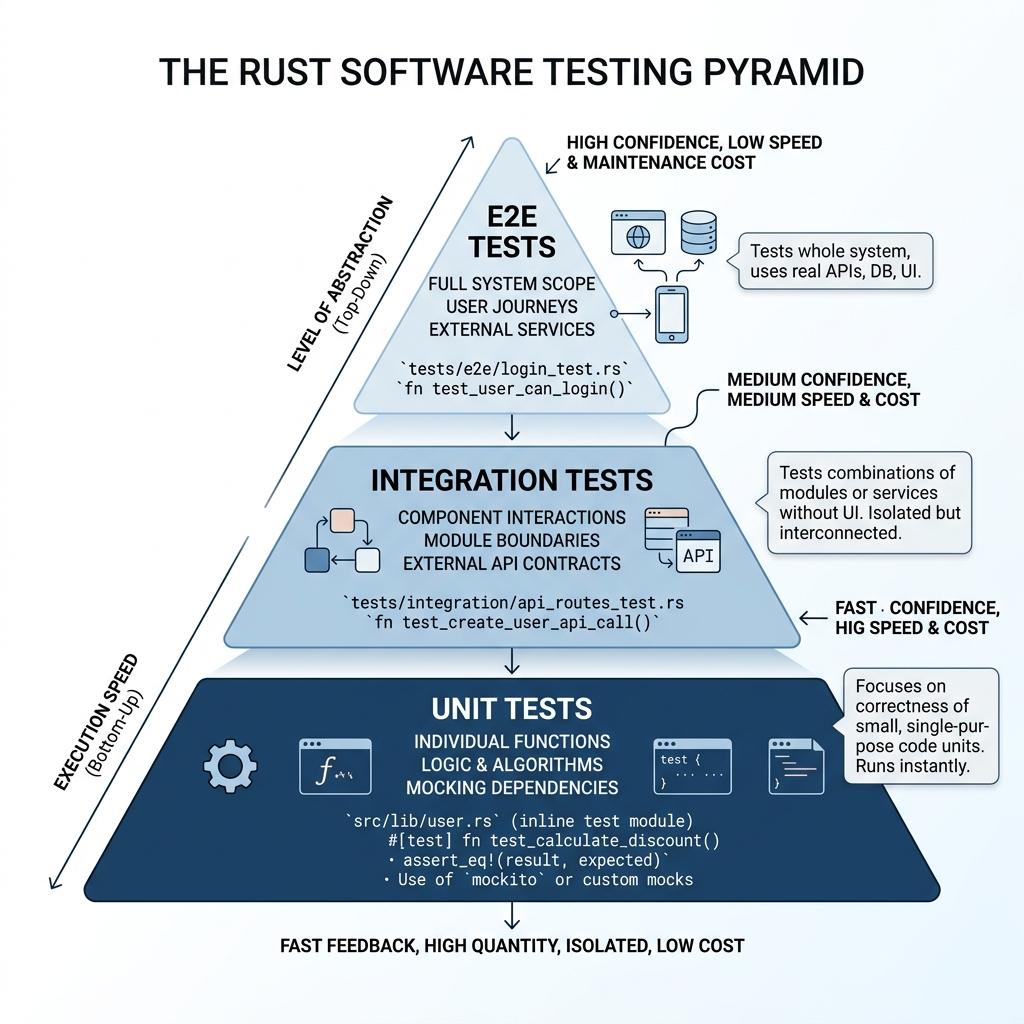
\includegraphics[width=0.7\textwidth]{images/testing_pyramid.png}
    \caption{The Testing Pyramid: Balancing cost, speed, and scope.}
\end{figure}

The pyramid consists of several layers:
\begin{itemize}
    \item \textbf{Static Analysis}: At the very foundation sits static analysis. In Rust, the compiler itself and tools like \texttt{rust-analyzer} or \texttt{clippy} catch numerous errors before the code even runs. As the professor distinguishes: "red flags" mean the code is broken, while "yellow flags" (warnings) indicate code smells or constructs written "as an intern" that should be simplified.
    \item \textbf{Unit Tests}: The base of the executable pyramid. These verify single, isolated elements of code. They answer the functional question: \textit{"Did we build the software right?"} They are fast, numerous, and written by the developer who knows the internal logic (\textit{white-box testing}).
    \item \textbf{Integration Tests}: The middle layer. These verify that multiple modules or systems work together correctly. They are essential when parts of a system (like a MySQL database) are out of our control and we must ensure our interactions with them are valid (\textit{black-box testing}).
    \item \textbf{End-to-End (E2E) Tests / Acceptance Tests}: The tip of the pyramid. These test the entire application from the user's perspective, answering the ultimate question: \textit{"Did we build the right software?"} (i.e., did we build what the client actually needed?). Furthermore, they evaluate operational criteria. As an analogy, if you buy a laptop, it is not enough that the CPU functions. It must weigh less than a kilo, the battery must last 4 hours, and it must have a backlit keyboard so you can use it at night. If it lacks these operational features, it is useless to the user, even if it is functionally flawless.
\end{itemize}

\section{Unit Testing: The Foundation}

Unit tests are aimed at checking if a single unit of code behaves exactly as expected in isolation. In Rust, writing and running unit tests is built directly into the language and its package manager, Cargo.

Because unit tests are typically written by the same developer who wrote the code, they are a form of \textbf{white-box testing}. You know the internal implementation details, which allows you to intelligently choose edge cases. As the professor illustrated: if you know a watch is mechanical (made of gears), you might test what happens if a grain of sand gets inside. If it is an electronic watch, sand might not affect it, but a drop of water would. Knowing the internal structure guides your testing strategy.

When writing unit tests, you must test the normal case (the "happy path") and the edge cases. To use another analogy: if you buy a car, you expect it to turn on. If it doesn't, you bought a stove, not a car. But you also need to know that the car still travels safely when it rains. If the car randomly evaporates into a pile of scattered iron pieces because of a thunderstorm, that is a severe failure. However, if you have a traditional gas car and you pour whiskey into the fuel tank, you \textit{expect} the engine to break. Testing edge cases means verifying both that the software survives realistic stress and that it fails predictably when misused.

This internal knowledge also highlights the importance of \textbf{cyclomatic complexity}---the number of independent paths through your code. If you have an \texttt{if} inside another \texttt{if}, you have 4 possible combinations. If that is nested inside a \texttt{for} loop, the number of combinations multiplies rapidly, creating what the professor calls "astral combinations" that can break everything. This is a strong incentive to keep functions small. It is far better to have two simple functions called in cascade than a single 200-line monolithic block, because smaller functions can be tested individually with ease.

Let's look at a trivial function that divides two numbers, and see how we would test it.

\begin{lstlisting}[language=Rust]
pub fn divide(a: i32, b: i32) -> i32 {
    a / b
}

#[cfg(test)]
mod tests {
    use super::*;

    #[test]
    fn test_divide_happy_path() {
        // Arrange
        let numerator = 6;
        let denominator = 3;

        // Act
        let result = divide(numerator, denominator);

        // Assert
        assert_eq!(result, 2, "6 divided by 3 should be 2");
    }
}
\end{lstlisting}

\textbf{Memory Model and Ownership Analysis:} In the \texttt{divide} snippet, both arguments \texttt{a} and \texttt{b} are primitives (\texttt{i32}). Primitives implement the \texttt{Copy} trait, meaning they are allocated entirely on the stack and copied into the function's scope when \texttt{divide} is called. There is no heap allocation or ownership transfer of dynamically allocated memory here. The \texttt{assert\_eq!} macro takes its arguments by reference behind the scenes (i.e., it borrows the \texttt{result} and the literal \texttt{2}), which is why it can compare them without consuming them, preserving their lifetimes if needed later in the test scope.

\subsection{Mechanism: The Test Module}
Notice the structure of the code above. We place our unit tests in a child module named \texttt{tests}. This module is annotated with \texttt{\#[cfg(test)]}. This is a conditional compilation flag: it tells the Rust compiler to completely ignore this module when compiling the application for release. The tests are only compiled and executed when you explicitly run the \texttt{cargo test} command.

Inside the module, we use \texttt{use super::*;} to bring the parent module's items (like the \texttt{divide} function) into scope. We then decorate individual test functions with the \texttt{\#[test]} attribute. The test runner uses this attribute to automatically locate and execute all test functions.

\begin{notebox}
\textbf{The AAA Pattern}\\
Notice how \texttt{test\_divide\_happy\_path} is structured into three distinct phases. This is known as the \textbf{Arrange, Act, Assert} (AAA) pattern:
\begin{itemize}
    \item \textbf{Arrange}: Set up the initial state, variables, and conditions.
    \item \textbf{Act}: Invoke the specific function or behavior under test.
    \item \textbf{Assert}: Verify that the actual outcome matches the expected outcome.
\end{itemize}
Adhering to this pattern keeps tests readable and consistent.
\end{notebox}

\begin{insightbox}
\textbf{Test Naming and "Furbo" Names}\\
It is crucial to give your test functions a "smart" (\textit{furbo}) name. Naming tests \texttt{t1}, \texttt{t2}, and \texttt{t3} is useless, because if \texttt{t3} fails, the test report tells you nothing about what broke. Instead, a name like \texttt{test\_when\_button\_clicked\_light\_turns\_on} gives you immediate context about what part of the application logic is failing.
\end{insightbox}

\subsection{Assertions and Usage Guidelines}
Rust provides a family of macros to verify outcomes. \textbf{When and why to use them:}
\begin{itemize}
    \item \texttt{assert!(condition)}: Use when you have a simple boolean outcome (e.g., checking if an \texttt{Option} \texttt{is\_some()}).
    \item \texttt{assert\_eq!(left, right)}: Use this as your primary verification tool. It compares two values for equality and, crucially, prints both values if the test fails. This makes it far superior to \texttt{assert!(a == b)} for debugging. 
    \item \texttt{assert\_ne!(left, right)}: Use when you want to guarantee state has changed or a value is not a default/error state, without knowing its exact new value.
\end{itemize}

When \texttt{assert\_eq!} fails, the error message indicates exactly what was expected versus what was found (e.g., "expected 7, found 5"). A common convention is to place the actual result on the left and the expected outcome on the right. A helpful mnemonic from the lecture is that the expected value goes on the \textit{right}, because in English, "right" also means "correct"!

\subsection{Advanced Testing Mechanics}
Beyond simple assertions, Rust allows test functions to return a \texttt{Result<(), String>}. If the test function returns \texttt{Ok(())}, the test passes; if it returns an \texttt{Err(String)}, the test fails, and the string is printed in the failure documentation. This is extremely useful when your test involves operations that can naturally fail using the \texttt{?} operator.

Additionally, within your \texttt{mod tests}, you are not limited to writing just \texttt{\#[test]} functions. You can write \textbf{auxiliary helper functions} to generate lists of inputs, construct complex objects, or generate random numbers to stress-test your domain space. For example, if you are testing floating-point math, a helper function could rapidly generate cases like \texttt{0.1 + 0.2} to check for precision issues.

\subsection{Testing Edge Cases and Failures}
Testing the ``happy path''---where all inputs are correct and everything works perfectly---is necessary but insufficient. You must also test \textbf{edge cases}. What happens if we pass zero as the denominator?

\begin{lstlisting}[language=Rust]
#[test]
#[should_panic(expected = "divide by zero")]
fn test_divide_by_zero_panics() {
    divide(6, 0);
}
\end{lstlisting}

If a function is structurally designed to panic under certain conditions, we can verify that behavior using the \texttt{\#[should\_panic]} attribute. If the function \textit{does not} panic, the test will fail!

\section{How Tests Drive API Design}

Writing tests often triggers an important psychological shift. When writing the \texttt{test\_divide\_by\_zero\_panics} test, a developer might realize: \textit{``Wait, if my function panics, the entire program could crash if user input happens to be zero.''} 

A test highlighting a panic condition is a strong signal that the function's signature might be flawed. In mathematics, division by zero is undefined. In software, we should embrace this complexity rather than ignoring it. 

Refactoring the code based on testing feedback leads to safer, more robust API design. Instead of panicking, the function should return an \texttt{Option<i32>} (or a \texttt{Result}):

\begin{lstlisting}[language=Rust]
pub fn divide_safe(a: i32, b: i32) -> Option<i32> {
    if b == 0 {
        None
    } else {
        Some(a / b)
    }
}

#[cfg(test)]
mod tests {
    use super::*;

    #[test]
    fn test_divide_safe_success() {
        assert_eq!(divide_safe(6, 3), Some(2));
    }

    #[test]
    fn test_divide_safe_by_zero() {
        assert_eq!(divide_safe(6, 0), None);
    }
}
\end{lstlisting}

\textbf{Memory Model and Ownership Analysis:} By returning an \texttt{Option<i32>}, the function still operates entirely on the stack. An \texttt{Option} is an enum, and since \texttt{i32} fits within standard processor registers/stack frames, no heap allocation is required. This makes the "safe" version just as memory-efficient as the panicking version, while cleanly transferring ownership of the result (the \texttt{Option}) back to the caller.

By writing the test, we discovered that our system was under-specified. We improved the design, making it the caller's responsibility to handle the \texttt{None} case. This results in software that is fundamentally safer.

\begin{insightbox}
\textbf{Tests as Documentation and Specification}\\
Working with clients is often a process of negotiation. A client might ask you to build a machine that separates egg yolks. Inside that machine, there will be tiny software sub-components that the client doesn't even know exist. You cannot ask the client how those microscopic internal pieces should behave in edge cases! You have to decide.

When you make these decisions, tests become a strict supplement to the specification. Instead of just remembering a vague conversation, capturing those requirements as executable tests is incredibly powerful. A test comment saying, \textit{``This edge case handles the specific scenario requested by Mario Rossi in his May 3rd email,''} prevents future regressions and ensures the specific requirement is never lost to time, even if someone else inherits your codebase.
\end{insightbox}

\section{Integration Testing}

While unit tests are excellent for testing specific logic in isolation (\textit{white-box testing}), they do not guarantee that the whole system works. What happens when multiple distinct components are assembled? 

This is where \textbf{integration tests} come in. Integration tests evaluate how modules interact. Because they test the interactions between components, they operate as \textit{black-box tests}. They cannot access the internal, private details of your modules; they can only use your library's public API, exactly as an external user would. 

To use an analogy from the lecture, consider testing a computer monitor. A unit test might verify in isolation that individual pixels turn on or that the HDMI decoder chip processes signals correctly. An integration test, however, treats the monitor as a black box: you send a video signal (input) and verify that the correct image appears on the screen (output). You do not look at the internal circuitry. Naturally, integration tests should only be run \textit{after} unit tests have passed; if you already know the display panel is broken, there is no point in checking the HDMI integration!

\subsection{Structure of Integration Tests}
In Rust, integration tests live outside the \texttt{src} directory, inside a dedicated \texttt{tests/} directory at the root of the project. Cargo compiles each file in the \texttt{tests/} directory as its own distinct crate. 

Imagine a system with two components: an \texttt{OrderRepository} that interacts with a database to fetch prices, and an application logic module that applies discounts. 

An integration test for this workflow might look like this:

\begin{lstlisting}[language=Rust]
// Inside tests/integration_test.rs
use my_store::repository::OrderRepository;
use my_store::services::DiscountService;

#[test]
fn test_applying_discount_updates_database() {
    // Arrange: Create an empty DB repository and populate it
    let mut repo = OrderRepository::new();
    repo.insert(1, 200.0); // Product ID 1 costs 200.0

    // Act: The service applies a 10% discount to product 1 (only if price > 100)
    let mut service = DiscountService::new(&mut repo);
    service.apply_discount(1);

    // Assert: Verify the repository reflects the new price (180.0)
    let updated_price = repo.find(1).unwrap();
    assert_eq!(updated_price, 180.0);
}
\end{lstlisting}

Notice how we are testing the assembled system as a \textbf{black box}. The integration test does not care \textit{how} the \texttt{OrderRepository} is implemented internally. It could be using a transient in-memory hash table (where data is lost when the program closes), or it could be connected to a robust, persistent MySQL database. The test simply presses the "buttons" of the public API and verifies the consequences.

\textbf{Memory Model and Ownership Analysis:} This integration test demonstrates complex borrowing dynamics. \texttt{OrderRepository::new()} allocates a \texttt{HashMap} on the heap, while the \texttt{repo} structure itself lives on the stack. When we call \texttt{DiscountService::new(\&mut repo)}, we create a mutable borrow of \texttt{repo}. The \texttt{service} instance holds this mutable reference, tying its lifetime to the mutable borrow of \texttt{repo}. Later, when we call \texttt{repo.find(1)}, we take an immutable borrow (\texttt{\&repo}). Why doesn't this cause a compiler error for having both a mutable and immutable borrow simultaneously? Because of Rust's Non-Lexical Lifetimes (NLL)! The mutable borrow held by \texttt{service} is no longer used after \texttt{service.apply\_discount(1)}, so the compiler gracefully ends the mutable borrow early, allowing \texttt{repo.find(1)} to safely take an immutable reference.

\begin{warningbox}
\textbf{The Cost of Integration Tests}\\
When an integration test fails, it is often more expensive to debug than a unit test. Because you are testing a complex flow across multiple modules, a failure means \textit{something} broke along the path, but the test doesn't explicitly tell you \textit{which} internal piece failed. Therefore, integration tests should supplement, not replace, a comprehensive suite of unit tests.
\end{warningbox}

\section{Parametric Testing with \texttt{rstest}}

Often, you want to test the same logic against many different inputs. Writing separate functions for each case can be tedious. Rust's ecosystem offers libraries like \texttt{rstest} to simplify this via parametric tests.

Using \texttt{rstest}, you define the parameters in the macro, and the test runner executes the function multiple times with the supplied data:

\begin{lstlisting}[language=Rust]
use rstest::rstest;

#[rstest]
#[case(6, 3, 2)]
#[case(10, 2, 5)]
#[case(-4, -2, 2)]
#[case(0, 5, 0)]
fn test_divide_multiple_cases(
    #[case] a: i32, 
    #[case] b: i32, 
    #[case] expected: i32
) {
    assert_eq!(divide(a, b), expected);
}
\end{lstlisting}

This centralizes the logic and clearly defines the expected input-output mappings without repetitive boilerplate. Additionally, if a specific test is currently broken but you want to run the rest of the suite without failure while you work on a fix, you can temporarily annotate it with \texttt{\#[ignore]}.

\begin{examprioritybox}
\textbf{White-box vs Black-box Testing}\\
The professor explicitly contrasts unit tests and integration tests. Unit tests are \textit{white-box}: you know the internal logic and can target specific nested `if` statements or edge cases. Integration tests are \textit{black-box}: you only see the public API, ensuring the assembled components interact correctly. 

\textbf{Common Pitfall:} Attempting to test internal implementation details within an integration test, or skipping unit tests because "integration tests will catch it."

\textbf{Expected Mastery Level:} High. You must be able to clearly distinguish between these two paradigms and know that integration tests go in a separate \texttt{tests/} folder and only test the public API.
\end{examprioritybox}

\section{The Limits of Testing: Concurrency and Proofs}

While tests are exceptional at finding bugs, they cannot definitively prove the \textit{absence} of bugs. You would need an infinite number of tests to cover every possible state of a non-trivial program.

This limitation becomes especially critical in \textbf{concurrent programming}. Concurrent programs depend on the flow of time and thread scheduling, which are non-deterministic and outside the programmer's control. A test might pass 99 times and fail on the 100th run simply because the threads happened to interleave differently. Therefore, for concurrency, testing is not enough. 

You must rely on logical demonstrations to mathematically ensure correctness, exactly like proving a geometry theorem. To prove the Pythagorean theorem, you start with Euclid's axioms (e.g., between two points there is a straight line) and logically deduce the truth. In concurrent programming, we use the axioms provided by the operating system (e.g., a Mutex can be possessed by only one thread at a time) and Rust's ownership rules to logically guarantee that data races cannot occur. Tests will help you catch glaring issues, but they cannot replace a sound logical proof.

\subsection*{Exam Relevance and Recurrence}
\textbf{Score: High}
Questions on testing often focus on the conceptual differences between unit and integration tests (white-box vs black-box), the location of test files, and conditional compilation flags (\texttt{\#[cfg(test)]}). You may also be asked to read a simple test and identify what makes it fail, or how a test-driven approach helps refine a function's signature (e.g., migrating from returning a panic to returning an \texttt{Option} or \texttt{Result}).

\section{Domande ed Esercizi da Esami Passati}

Nessuna domanda specifica per questo capitolo negli esami passati analizzati.

